%% $Id: residential_location_neighborhood_dynamics.tex,v 1.1 2006/01/30 21:12:09 pwaddell Exp $

\documentclass[12pt,a4paper]{article}

\usepackage{txfonts}
\usepackage[T1]{fontenc}
%\usepackage[latin1]{inputenc}

\usepackage{array}
%\usepackage{lscape}
\usepackage{rotating}
\usepackage{longtable}
\usepackage{lscape}
%\usepackage{natbib}
\usepackage{url}
\usepackage{graphicx}
\usepackage{supertabular}

%
% Change coordinates to edge of page
\voffset=-1in \hoffset=-1in
%
% Set for US Letter
\textheight=9.5in \textwidth=6.5in \topmargin=0.5in
\oddsidemargin=1in \evensidemargin=1in
%
\frenchspacing \raggedbottom
%\renewcommand{\thesection}{\Alph{section}}
%\renewcommand{\theenumii}{\arabic{enumii}}

%\newcommand{\ve}[1]{\mathbf{#1}}
\newcommand{\vk}[1]{\mbox{\boldmath $#1$}}
\newcommand{\tight}{\itemsep 0pt}

\begin{document}

\title{Residential Location and Neighborhood Dynamics}

\author{\\
Paul Waddell\\
Evans School of Public Affairs, University of Washington,\\
Box 353055, Seattle, WA 98195 \\
( 206) 221-4161, pwaddell@u.washington.edu} \maketitle


\baselineskip=.3in

\begin{abstract}
\baselineskip=.3in

The choice of residential location by individual households
determines many aspects of the quality of the social, economic and
physical environment experienced by its members, and there are
well-documented adverse effects of living in neighborhoods with
high concentrations of poor and racial minorities.  We seek to
analyze the processes of household choice of residential location,
and the neighborhood dynamics that emerge from these individual
choices.  Unfortunately, analysis of this choice process is
complicated by the endogeneity of neighborhood social composition,
housing prices, housing supply, and even of the spatial pattern of
access to employment. This paper describes an effort to gain new
analytical insights into the relationships between individual
household choices and emergent outcomes by developing disaggregate
discrete choice models and linking them in an agent-based
simulation system. The framework is developed and applied to two
cases, a simple model neighborhood change, and a more ambitious
model system that incorporates multiple processes endogenously,
including residential location, housing supply, prices, job
location, and travel.  A new open-source platform for
specification, estimation and simulation of models in this genre
is described.

\end{abstract}
\clearpage

\section{Introduction}

Problems associated with neighborhood racial segregation and
concentration of poverty, and the dynamic processes of
neighborhood decline, and at times revitalization or
gentrification, have been subjected to sustained academic research
from various social science perspectives over many decades. Yet
significant issues remain difficult to address in this research
domain, which lies at the intersection between microscopic
perspectives that focus on individual choices such as residential
location, and macroscopic perspectives that focus on the aggregate
dynamics and emergent spatial patterns across neighborhoods.  The
extensive research assessing neighborhood effects on individual
outcomes such as employment or dropping out of high-school
attempts to link these micro and macro perspectives by examining
how the neighborhood context shapes individual experiences.  There
is relatively little research, on the other hand, that attempts to
explore neighborhood dynamics by analyzing the dynamic choices of
individuals.

The issues of neighborhood segregation and dynamics lie at the
intersection of several lines of research, including work on the
urban underclass (Wilson, 1987), the suburbanization of employment
opportunities and the resulting 'spatial mismatch' of jobs and
inner-city poor blacks (Kain, 1968), economic restructuring that
is eliminating high paying manufacturing jobs in the central city
and creating high paying knowledge sector and low paying service
jobs (Kasarda, 1985), the filtering of housing from higher to
lower socioeconomic levels producing abandonment in the poorest
inner-city neighborhoods (Stegman, 1977), racial preferences in
residential location (Clark, 1992), racial and economic
segregation (Jargowsky, 1996), and the spatial assimilation of
racial minorities (Massey, 1981). The concentration of urban
poverty has intermittently captured national concern, particularly
after watershed events such as the riots in southern Los Angeles.
The issue is once again a focus of policy debate and research
activity.

A growing body of research has highlighted the adverse
consequences of living in poor neighborhoods. Wilson (1987) has
argued that concentrated male black joblessness isolates ghetto
residents from the world of work, and promotes a culture of
dependency. According to Massey and Shibuya (1994), concentration
of  male joblessness leads to higher probabilities of joblessness
among young black men, and lower rates of marriage among black
women. Jencks and Mayer (1990) review a number of studies
examining the broader consequences of poverty concentration.
Spatial analysis of poverty concentration has tended to focus on
rates of racial segregation, which have been shown by Farley and
Frey (1994) to be declining since 1970, and economic segregation,
which according to Jargowsky (1995), have been increasing across
and within racial groups since 1970.

A rapidly growing literature has approached the analysis of
emergent properties of individual agent choices by developing
Agent-Based Models (ABMs). Using relatively simple rules to govern
the behavior of agents that are influenced by their immediate
surroundings, ABMs are making significant inroads as a research
method in sociology, political science and economics, among other
fields (Epstein and Axtell, 1996; Axelrod, 1997; Macy and Willer,
2002; Tesfatsion, 2006). Drawing on the emergence of widely
available software tools to develop agent-based models such as
Swarm, Repast and Sugarscape, and stimulated by Schelling's (1969,
1971) pioneering work on segregation as an emergent outcome of
individual choices based on weak preferences, recent work has
begun to develop and test theoretical propositions regarding the
emergence of racial segregation using ABMs (Bruch and Mare, 2004;
Fosset, 1999; O'Sullivan, Macgill and Yu, 2003).  The literature
emerging from this approach is principally of a theoretical
nature, with relatively few attempts to empirically test these
models against observed data.  Model parameters in the ABM
literature are generally assumed rather than estimated from data.

A different approach to modeling individual actions using discrete
choice models emerged in the 1970's, with the pioneering work of
McFadden on Random Utility Maximization theory (1973). This
approach derives a model of the probability of choosing among a
set of available alternatives based on the characteristics of the
chooser and the attributes of the alternative, and proportional to
the relative utility that the alternatives generate for the
chooser. Maximum likelihood and simulated maximum likelihood
methods have been developed to estimate the parameters of these
choice models from data on revealed or stated preferences, using a
wide range of structural specifications (see Train, 2003). Early
application of these models were principally in the transportation
field, but also included work on residential location choices by
Lerman (1977), McFadden, (1978), and Quigley (1976) among others.

In this paper, I undertake the problem of analyzing neighborhood
dynamics by drawing the discrete choice modeling on a different
literature, one that focuses on modeling choice behavior using
discrete choice models, as pioneered by McFadden (1974). Using
disaggregate choice models empirically estimated from observed
data, I explore the degree to which important neighborhood
patterns and dynamics can be predicted from microscopic modeling.
In the process of developing these models, I address problems of
endogeneity that plagues research on neighborhoods, raising
several and partially addressing them.

The paper is organized in two parts.  The first part develops a
simpler longitudinal model that focuses on capturing essential
elements in the dynamics of neighborhood concentration by race and
poverty status, with an application to census tracts in the
Dallas-Forth Worth metropolitan area from 1970 to 1990.  The
second part of the paper describes a more extensive modeling
effort to predict residential location choices at a microscopic
scale, as part of a broader simulation model system that also
endogenizes housing prices, housing supply, and firm location.
This model system has been created using a new open source
simulation software package that is briefly described.  The paper
concludes with a summary of the main contributions and suggestions
for further research.


\section{Dynamics of Neighborhood Poverty Concentration}




\section{Drivers of Neighborhood Dynamics}

For such rapid population dispersal to occur, the housing market
must have produced an overabundance of new housing at the urban
periphery, causing housing costs to fall, and affording mobility
opportunities to households wishing to move to more suburban
locations. The classical process of housing filtering described by
Lowry (1960) and Stegman (1977) is characterized by upper income
households moving into new housing at the periphery, vacating
their older and somewhat devalued prior residences to be occupied
by households usually with lower economic status, who in turn,
vacate their housing to be occupied by households of yet lower
status, until the vacancy chain results in abandonment of the
least desirable housing in the inner city.

The housing filtering process appears to be at work with a
vengeance in the past two decades in the Dallas-Fort Worth area.
The number of housing units increased by 598,000 in the
Dallas-Fort Worth area from 1970 to 1990, outpacing the increase
of 566,000 households. As a result of rampant overbuilding and a
mid-1980's recession, vacant housing increased from 45,000 in 1970
to 146,000 in 1990, an increase of 227\%. During such soft housing
market conditions, it should be expected that the housing
filtering process would accelerate sharply. The spatial
distribution of the housing stock over the 1970 to 1990 period
also reveals that there was significant housing removal from the
core high poverty areas, with a cumulative loss of 27\% of the
housing stock from census tracts that had a 40\% or higher poverty
rate in 1990. There was a slight loss of housing even in
borderline neighborhoods with 1990 poverty rates between 30\% and
40\%. On the other hand, housing increased by 182\% between 1970
and 1990 in the census tracts below 10\% poverty in 1990. Given
this dramatic rearranging of the housing opportunity set brought
about by self-interested developers, coupled with underlying
tendencies for suburbanization, the dispersal of poor population
was accelerated to a pace no governmental program or incentive
would have been likely to match.

The detrimental influence of suburbanization of employment on
unemployment outcomes for blacks living in segregated inner city
ghettos was identified by Kain (1968) as the spatial mismatch
hypothesis. It has been argued by Ellwood (1986) and others that
the black-white employment rate gap is more due to racial
discrimination than spatial isolation, or "race, not space."
Ihlandfeldt and Sjoquist (1990) found in a study of Philadelphia
that between a third and a half of the gap between black and white
employment rates can be explained by lower accessibility to
employment by blacks.  Kasarda (1985) has also explored the effect
of the loss of  employment base, particularly in lower-skill
industries such as manufacturing, on the economic outcomes of
blacks. In this section, we examine trends in employment location
with respect to the geographic expansion of the high poverty area.
The employment data are from the North Central Texas Council of
Governments, which compiled the data from establishment listings
and census journey to work tabulations from each decennial census.
In Table 3, the employment totals for major industrial groups are
presented within the same fixed geographic boundaries used in the
preceding analysis.

The employment trends clearly distinguish a dramatically lower
rate of employment growth within the high poverty areas compared
to low poverty areas.  Total employment, for example, grew three
times faster from 1970 to 1990 in the census tracts that had a
1990 poverty rate below 40\% than those over 40\%.  This ratio
grows to five to one when comparing job growth in census tracts
with under 10\% poverty to those over 40\% poverty in 1990.  In
sectors particularly important for low income workers, such as
manufacturing, the high poverty areas lost 17\% of their job base,
while census tracts below 40\% poverty gained 31\%, and census
tracts below 10\% poverty gained 59\% in manufacturing employment.
Wholesale trade exhibited virtually no growth in the high poverty
areas, but grew by 107\% in census tracts below 40\% poverty in
1990, and by 256\% in census tracts below 10\% poverty in 1990.
In the retail and service sectors, while  growth appeared to occur
within the high poverty neighborhoods, it also was overwhelmed by
the growth in low poverty neighborhoods.  Only in government
employment, which tends to be centrally located with city, county,
state, and federal employment in or near downtown Dallas and Fort
Worth, did this trend not hold.

\section{Simulation of Household Location and Emergent
Neighborhood Dynamics}

While the preceding regression analysis sheds some light on the
dynamics of neighborhood change, a more compelling approach would
be to generate these dynamics by simulating individual household
choices to relocate within the housing market.  This section
develops such a microsimulation model, beginning with mobility and
then turning to location choices. MOBILITY The key to the proposed
model is that the evolution of neighborhood composition over the
twenty-year period of study can be decomposed into two components:
1)  Population residing in each neighborhood make mobility
decisions with the outcomes being: remain in the same neighborhood
(don't move), move to a new neighborhood within the metropolitan
area, or move out of the metropolitan area.  Population in other
metropolitan areas are of course making similar choices, with some
pool of migrants eventually choosing to relocate to the
metropolitan area of focus. 2)  Once decisions are made to move,
persons choose locations in neighborhoods from the available set
of housing vacancies, in a way that maximizes their utility based
on the bundle of characteristics of the available housing and its
neighborhood. The dynamics of these two choices, propagated over
time across the population at large, results in an evolution of
the racial and socioeconomic composition of each neighborhood, as
well as an aging of its housing stock.  In some neighborhoods, the
changes will be modest, with out-migrating households replaced by
similar households and little compositional shift.  In other
neighborhoods, differential rates of out- and in-migration between
the various types of population result in compositional shifts
that are at times dramatic, and perhaps more often, gradual but
inexorable.  The combination of the decision to move and the
choice between alternative neighborhood locations, then, though
made by individual households, quickly affect the aggregate
compositional outcomes at the neighborhood level.  In turn, these
compositional shifts alter the preferences of potential
in-migrants, either dampening or accelerating the transition
already underway. Research on mobility suggests that household
characteristics, and changes in those characteristics over time,
go a long way toward explaining the residential mobility decision.
Among the characteristics likely to influence move decisions are
age, family structure, socioeconomic status, and potentially,
race.  This study faces data limitations with regard to the
household characteristics, since it is based on census tract level
data from 1970, 1980, and 1990, and a relatively small number of
joint distributions of population characteristics are available at
the tract level in any one census year, let alone consistently
across three census years.  The categorization of population into
three racial groups, stratified into above and below poverty,
provides the only population characteristics for which we have
obtained a consistent joint distribution (race by income) across
all three census years.  We therefore do not have information
about household structure and age of head, both of which are
valuable in predicting mobility choices.
Nevertheless, we do find significantly different mobility rates across these six categories of population, and these are used as the basis for developing the pool of movers in each time interval.  Using the Public Use Microdata Sample (5%) for 1990, we analyze questions pertaining to mobility over the prior five year interval, by race and poverty status.  Since the mobility rates we are interested in are out-migration rates, and the census reports migration retrospectively over five years, we need to use 1985 as our base year for estimating migration rates, and must identify those persons that moved out of the metropolitan area between 1985 and 1990.  We therefore scanned the entire U.S. PUMS data, retrieving all records in which persons reported having moved from one of the Public Use Microdata areas (PUMA) within the Dallas-Fort Worth metropolitan area, to add them to the pool of residents that remained in the metropolitan area between 1985 and 1990.  We also subtracted out those persons who moved into the area during that time.
Results of this tabulation are shown below, in Table 1. Table 1:
Mobility Rates by Race and Poverty Status
    Mobility Rate 1985-90
Population Group    Moved Within Dallas-Ft Worth    Moved out of
Area   Total Out-migration Rate
White Above Poverty 33.9%   18.9%   52.8%
Black Above Poverty 42.6%   9.3%    51.9%
Other Above Poverty 44.1%   13.4%   57.5%
White Below Poverty 34.7%   36.9%   71.6%
Black Below Poverty 50.3%   10.2%   60.5%
Other Below Poverty 51.1%   19.1%   70.2%

These mobility rates are fairly consistent at the aggregate level, with 52% to 58% of the population above poverty in Dallas-Fort Worth moving, and 61% to 72% of the poor population moving within the same time period.  The higher mobility rates among poor are probably related at least in part to a higher probability that poor persons rent rather than own their homes, and to a disproportionate representation of young persons, which tend to have substantially higher mobility rates than older persons, in the poor population group.  Across races, it appears that the overall migration rate for Blacks is lowest among the three groups, though the gap for above poverty Blacks is unlikely to be significant.  The mobility rate among poor Blacks is about 10 percentage points below either White of Other poor population, which may be a combination of lower average incomes even within the poor category which limits relocation opportunities, higher probabilities of residence in public housing, and potential discrimination in the housing market.
The internal composition of these migration rates between moves within the metropolitan area and moves out of the metropolitan area reveal larger differences between groups.  Roughly one third of Whites above and below poverty moved within the metropolitan area, while close to 45% of non-poor Blacks and others, and 50% of poor Blacks and others did so.  Both above and below poverty Whites were more likely to move out of the metropolitan area than either Blacks or others, with the largest differences between poor Whites (37%) and poor Blacks (10%).  The poor White out-migration may be related in part to the historical artifact that the Dallas economy went into a massive recession in the latter 1980's, after having experienced a major economic boom in the early 1980s.  The rapid increase in blue collar jobs, followed by a rapid loss of those same jobs, particularly in the construction industry, may have stimulated a wave of in-migration of blue-collar workers in the early 1980's followed by a large exodus in the latter half of the decade.
We use these total migration rates as the basis for predicting
out-migration from each census tract during the period,
recognizing that they are only a first approximation.  Data were
not readily available to repeat these tabulations for 1970 and
1980.  That will be done at a later date. RESIDENTIAL LOCATION In
modeling the residential location choices made by within-area
movers and in-migrants to the metropolitan area, we seek to
combine elements from several theoretical approaches.  First, the
concept of housing filtering described by Muth (1969) and others
suggests that upper income households will tend to occupy new
housing constructed at the urban periphery, initiating a chain
reaction of vacancies as their previous housing becomes occupied
by slightly lower income households moving up from lower-income
neighborhoods, which in turn creates more vacancies in lower
income neighborhoods, ultimately culminating in the abandonment of
housing in the poorest and least desirable neighborhoods, for
which there is insufficient demand to fill the available housing.
In the proposed model, we treat the supply of new housing as
exogenous, and divide the housing available into new housing built
in the most recent period, and existing housing from the previous
period, since the utility of new and older housing are likely to
differ for poor and non-poor households.  Ideally, we would use
housing prices and incomes to establish a market clearing price
adjustments and impose budget constraints on residential location,
but our data are insufficiently detailed to allow this, and we use
the new and existing housing in combination with the poverty rate
in the neighborhood, which we predict endogenously, as proxies for
housing prices and incomes. There is a broad range of theoretical
and empirical literature pertaining to the racial and economic
sorting processes of households, including tipping models of
racial change (Bailey,1959), models of spatial assimilation of
Blacks and Hispanics (Massey,1981), studies on racial preferences
in residential location (Clark, 1992), the long tradition of
social and factorial ecology and its identification of race,
socioeconomic status and life cycle as primary determinants of
residential location (Berry and Kasarda, 1977), and research on
segregation rates by race and class (Jargowsky,1996).  We seek to
implement in this model a simple mechanism to measure and make
endogenous many of these effects.  Our strategy is to predict the
mobility and locational choices of persons by race and poverty
status, which we can aggregate at the neighborhood level to
dynamically update the racial and economic composition of each
neighborhood.  To the extent that our six categories of
population, stratified by race and poverty status, capture at
least the broad dimensions of racial and economic sorting, the
model will allow us to examine the relative strength of the
sorting processes of these household types over a twenty year
period, controlling for the distribution of existing and new
housing opportunities, and the distribution of existing and new
jobs, to which we now turn. Job access has traditionally played a
dominant role in models of residential location, with the prime
examples being the monocentric model and its successors (Alonso,
1964; Muth, 1969; Mills, 1970), and the spatial interaction models
(Lowry, 1964; Putman, 1983; Wilson, 1967).  Both of these modeling
traditions assume that residence choices are made based on an
exogenous choice of workplace.  That is, once we know a person's
workplace, we predict their residence location on the basis of
commuting time or distance to work, and attributes of residential
locations such as housing quality or price.  A growing body of
work has questioned the validity of this assumption, suggesting
that residence and workplace choices are not, on balance,
consistent with the exogenous workplace assumption (Waddell,
1993a,; Merriman, 1994).  Instead, it would appear that factors
such as multiple-worker households have made the
residence-workplace connection as amenable to assumptions of
joint-choice or independent choice.  Some have even suggested that
the sequence of choices may be the reverse of the traditional
workplace-residential location sequence (Steinnes, 1977). In other
work, the sequence of choices of residence location, workplace,
and housing tenure for single-worker households have been modeled
jointly (Waddell, 1997).  In this paper, we take a different
approach by de-coupling the choice of residence and workplace, in
order to focus more thoroughly on neighborhood dynamics that
emerge from agent-level mobility and residential location choices.
Rather than assume that residential choices are conditional on
prior workplace choices, we relax this assumption to allow persons
to choose residential locations within a metropolitan area on the
basis of the availability of new and existing housing, the racial
and economic composition of the neighborhood, and generalized
accessibility to job opportunities in broad economic sectors such
as basic, retail and service industries. This relaxation of the
exogenous workplace assumption is potentially a more realistic way
to analyze the locations of multiple-worker households that must
juggle more than one workplace commute, and are unlikely to
minimize the commute of the 'head of the household,' a concept
that has become difficult to rationalize.  In addition, some
research suggests that the role of workplace accessibility in
residential location may be substantially less than traditionally
thought.  One reflection of this is that non-work trips now
comprise three of every four workday trips, making the workplace
commute relatively less important in the overall accessibility of
households (Richardson and Gordon, 1989). We implement the
proposed approach by measuring the accessibility to jobs by type
from each residential location, in our case the normalized census
tract.  The accessibility indices for each employment sector are
calculated using a standard distance weighting, or gravity
formulation:
 ,
where   EmpAccik is the employment access index for zone I to
employment in sector k Ejk is employment in zone j in sector k,
    dij is the Euclidean distance between the centroid of zone I and zone j.
Although travel time or cost as a discounting measure might have
been preferable, such data were not available for 1970, 1980,  and
1990, and it is likely that these distance measurements would be
highly correlated with those alternative measures. A final issue
with respect to the measurement of the neighborhood
characteristics entering the models of location choice is that
most models treat the zones of residential location as totally
independent units.  Each census tract (or other neighborhood
boundary) is treated as an isolated observation with no shared
attributes with adjacent or nearby neighborhoods.  The recent
development of the field of spatial econometrics (Anselin,1988)
has shown that failure to account for spatial autocorrelation
across zones can bias results.  In addition, with respect to
theories regarding neighborhood tipping (racial or economic), we
would expect that changes in adjacent or nearby neighborhoods
could figure prominently in the mobility and residential location
choices of current and prospective residents of a given
neighborhood.  The accessibility measurements for employment
described above provide an approach that can be applied to the
racial and economic composition of the area surrounding each
census tract, thereby allowing us to measure the effects of
changes in nearby census tracts on preferences for location. The
first step in constructing these broader compositional measures is
to compute accessibility indices to population by type in the same
way they were computed for employment:
 ,
where   PopAccik is the population access index for zone i to
population of type k Pjk is population in zone j of type k,
    dij is the Euclidean distance between the centroid of zone I and zone j.
The relative composition of the surrounding area can then be
computed as the percentage of a particular group or groups of the
total population accessibility index.  In this way, we compute the
poverty rate and percent Black within a broader neighborhood
context.  In addition, when we apply the model dynamically over
time, we endogenously update these accessibility indices and
compositional measures based on our predictions of residential
location by race and poverty status. With this description of the
independent variables in the residential location model, we
proceed to describe the model structure.  The model is based on
random utility theory, and draws on a growing body of research
using discrete choice models to predict choices from among a set
of discrete alternatives (McFadden, 1973).  More recent research
activity has included numerous additional applications to mode
choice, but also to residential location.  Such applications of
the multinomial logit model include a the demand for housing by
rental households in Pittsburgh (Quigley, 1976), estimation of
housing submarket demand equations for renters and owner-occupants
in the Chicago and Pittsburgh housing markets (Apgar and Kain,
1974), residential destination choice (Lerman, 1977; McFadden,
1978),  joint residential location and travel mode choice (Anas,
1981), and housing demand and tenure choice components of the HUDS
housing market simulation (Kain and Apgar, 1985), and choices of
residence, tenure, and workplace (Waddell, 1993a, 1993b, 1996).
This model differs from these and other earlier models in that its
intent is to model the residential location choices of only recent
movers, once they have made the decision to move, and to link the
mobility and location choices into a dynamic simulation model, as
has been done in a (Waddell, 2000, 2002). We assume individuals
will attempt to maximize their utility in their choices of
residential location.  Total utility is then separated into
deterministic and random components
 ,
where Vin is the systematic, or deterministic component of the
utility of alternative i for individual n, and  in is the random
component of the utility. We use the multinomial logit, or
discrete choice model, to predict the probability that individual
n will choose alternative i, based on the relative attractiveness
of the alternative compared to all others:
 ,
where   is the feasible choice set for individual n. The
systematic component of the utility function is specified as:

where   TOTHU is the total housing units in census tract i,
    HUCH is the change in total housing units from the prior time period in tract i,
    PCTBLK is the percentage Black population in census tract i,
    PCTOTH is the percentage Other population in census tract i,
    PCTPOV is the percent of the population below poverty in census tract i,
    LAPOP is the log of the population accessibility index for the previous time period,
    PBLKA is the percentage BLACK of the population accessibility index,
    PPOVA is the percentage below poverty of the population accessibility index,
    LABAS is the log of the employment accessibility index for basic employment in the previous time period,
    LARET is the log of the employment accessibility index for retail employment in the previous time period,
    LASER is the log of the employment accessibility index for service employment in the previous time period,
    ABASCH is the change in the employment accessibility index for basic employment from the previous time period,
    ARETCH is the change in the employment accessibility index for retail employment from the previous time period, and
    ASERCH is the change in the employment accessibility index for service employment from the previous time period.
Since our application involves choices among more than 300
normalized census tracts, we employ a convention of random
sampling of alternatives to make the estimation of model more
tractable.  The independence of irrelevant alternatives property
permits the use of a sample of alternatives in specifying a
multinomial logit model with a large number of alternatives.
McFadden (1978) established a positive conditioning property as a
condition for a consistent estimator for the logit model with
samples of alternatives, and uses it to prove that maximization of
a conditional log likelihood function yields consistent estimates
of the unknown parameters under normal regularity assumptions (see
also Ben-Akiva and Lerman, 1987). We have data on the joint
distribution of the population in each census tract by race and
poverty status, and estimate the location choice model using the
1990 population distribution by type, discounting the totals
within each census tract by the fraction of the total population
that moved into the census tract within the past five years to
approximate the number within each group that were recent
migrants.  Since the mobility question was not cross-tabulated
with any other variables in the census tract data available from
the census, we make the assumption that the same fraction of each
of our subgroups within the census tract moved in during the past
five years. Results of the residential location choice model
estimation are given in Table 2, below, and the parameter
estimates are compared across the six population groups in Figure
1. The signs and relative magnitudes of the parameter estimates
appear plausible and consistent, and a large majority of the
asymptotic z statistics are significant.  The overall goodness of
fit of the models is given in Table 3, below. Table 3: Goodness of
Fit Measures for Location Choice Models Model   Observations
Log-likelihood  Log-likelihood with No Coefficients White Above
Poverty 2023    -747.5  -1042.2 White Below Poverty 2023
-1002.4 -1042.2 Black Above Poverty 2023    -878.4  -1042.2 Black
Below Poverty 2023    -991.7  -1042.2 Other Above Poverty 2023
-1018.9 -1042.2 Other Below Poverty 2023    -1048.3 -1042.2



\section{UrbanSim}

The resulting modelling framework had several key design features
\cite{waddell-env-and-planning-2000,waddell-japa-2002}, all of
which have been subsequently promoted by others in the research
community as elements of an `ideal' model system
\cite{miller-tcrp-1999}:


\begin{itemize}

\item Agent-level representation: individual households and jobs

\item Dynamic representation of time, usually in annual steps,
with path-dependence

\item Representation of highly disaggregate geographies, such as
small grid-cells or parcels

\item Representation of individual choice processes: moving,
locating

\item Use of a discrete-choice modelling framework to represent
choice behavior.

\item Representation of interactions of households, firms and
developers in real estate markets, and the role of prices.

\item Representation of \emph{scenarios} of public policies for
land use, transportation and the environment .

\end{itemize}

UrbanSim models household residential location choice, employment
location choice, and real-estate development choice models as
discrete choice models, drawing on the Random Utility Maximization
(RUM) framework pioneered by Daniel McFadden, who won a Nobel
Prize in Economics for this and related work
\cite{mcfadden-1974,mcfadden-1981}. For each agent, we assume that
each alternative $i$ has associated with it a utility $U_i$ that
can be separated into a systematic part and a random part:
\begin{equation}
    U_i = u_i + \epsilon_i,
    \label{eq:utility}
\end{equation}
where $u_i = \vk{\beta}\cdot\vk{x}_i$ is a linear-in-parameters
function, $\vk{\beta}$ is a vector of $k$ estimable coefficients,
$\vk{x}_i$ is a vector of observed, exogenous, independent
alternative-specific variables that may be interacted with the
characteristics of the agent making the choice, and $\epsilon_i$
is an unobserved random term. Assuming the unobserved term in
(\ref{eq:utility}) to be distributed with a Gumbel distribution
leads to the familiar multinomial logit model
\cite{mcfadden-1974,mcfadden-1981}:
\begin{equation}
    P_i = \frac{\mathrm{e}^{u_i}}{\sum_j \mathrm{e}^{u_j}},
    \label{eq:mnl}
\end{equation}
where $j$ is an index over all possible alternatives. The
estimable coefficients of (\ref{eq:mnl}), $\vk{\beta}$, are
estimated with the method of maximum likelihood (see for example
\cite{Greene-2002}).

Within the UrbanSim model system, the choice process proceeds as
shown in Figure \ref{fig:choiceprocess}.

\begin{figure}[h]
\center
 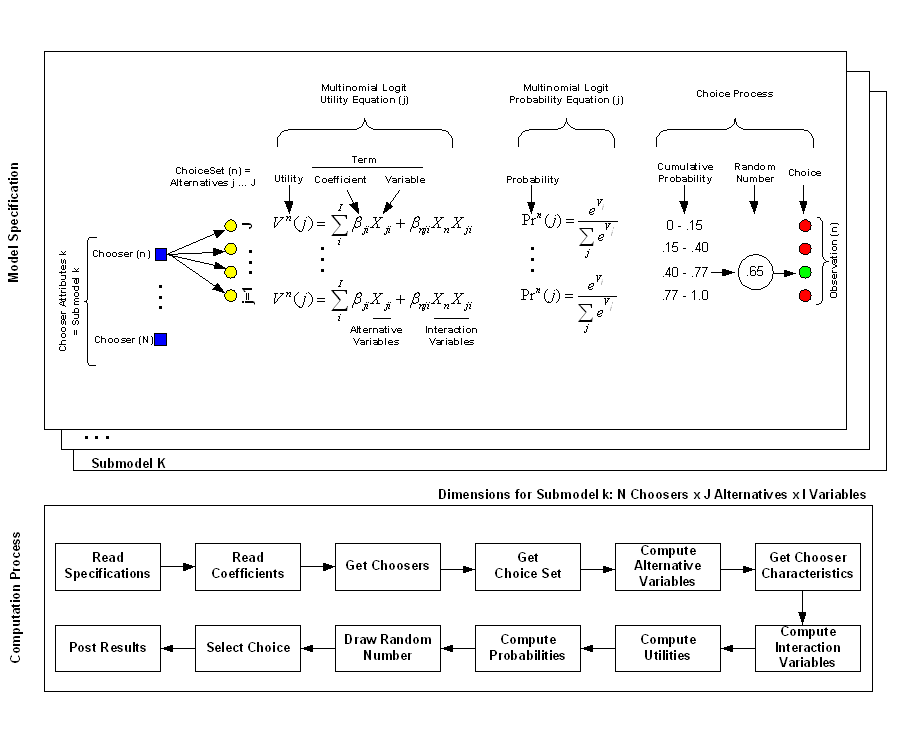
\includegraphics[width=6.5in]
 {ChoiceProcess.png}
\caption{Choice Process in UrbanSim Location Choice Models}
\label{fig:choiceprocess}
\end{figure}

The first steps of the model read the relevant model
specifications and data.  Then a choice set is constructed for
each chooser.  Currently this is done using random sampling of
alternatives, where alternatives are grid cells of 150 meters by
150 meters, and the cells are weighted by the number of locational
opportunities in them (vacant housing for the residential location
choice model).  Note that this sampling method has been shown to
generate consistent, though not efficient, estimates of model
parameters \cite{ben-akiva-lerman-1987}.

Once the choosers (movers or new households) are selected and the
choice sets of alternative locations sampled, the relevant
variables used in the utility function are computed.  For
efficiency, this proceeds by computing characteristics of
alternatives first for all alternatives in the universe, then
computing interaction terms for only the set of choosers and their
sampled locations.  After this, the logit calculations predict
probabilities for all the available choices in the choice set for
each chooser.  Finally, the process makes a selection by drawing a
random number, comparing it to the cumulative distribution of the
predicted alternatives, and selecting the choice which the random
draw falls within.  At this point the choice is posted to the
database for the chooser, and the number of available housing
units is reduced by one to reflect that the unit is no longer
vacant.

Household agents have characteristics of race, income, size,
presence of children, age of head, number of workers, and number
of vehicles. The initial base year population is derived from
census data using a synthetic population procedure
\cite{beckman-1995}, which uses Iterative Proportional Fitting to
scale the joint probability distribution of household
characteristics in the Census Public Use Microdata 5\% Sample to
the marginal distributions available by census tract and block
group from Census Summary File 3. A sample of real households is
used for model estimation, generally taken from regional surveys
for transportation planning.  These surveys provide detailed
geocoding to allow assignment of locational characteristics to
sample households, which is essential for estimating location
choice models.

Firms are represented in UrbanSim at the level of individual jobs,
with the sector of the firm and the location of the establishment.
Typically, public sources of employer data from unemployment
insurance records have been used to generate an inventory of
business establishments for model application.

Information on individual land parcels is obtained from individual
tax assessor offices and compiled into a regional database.
Considerable imputation and cleaning of these data are often
needed, to address gaps and inconsistencies in the data, such as
tax-exempt properties.  The attributes generally include year of
construction, type of development, square footage of building,
land area, land use classification, and land and improvement
(building) values.  These data are then transformed into a grid
representation for model development purposes, combining parcel
fragments that fall into the same grid cell and assigning an
overall development type classification to the cell.  Quantities
of housing and nonresidential square feet are retained for
accounting of occupancy by households and jobs.  A detailed
discussion of the data integration process is available
\cite{waddell-cuspa-2004}.

The need to run the model in operational contexts ranging from
small to large metropolitan regions, and representing individual
households, jobs and small grid cells, led to significant
challenges in the software design and implementation.  Java was
used as the development language, but its object overhead required
too much memory to scale well to larger regions on standard
desktop computers.  To address this, a design of exploded objects
was used to retain an object representation, but using an internal
storage mechanism of parallel arrays.  Another key design element
in the software architecture was the use of implicit invocation to
manage communication by modular model components entirely through
their interaction with a data store \cite{noth-ceus-2003}.  In
addition to these techniques to improve efficiency, substantial
caching was used to avoid redundant computing.

UrbanSim has now been applied in several metropolitan regions,
including Eugene-Springfield, Oregon, Honolulu, Hawaii, Houston,
Texas, Salt Lake City, Utah, and Seattle, Washington, and has been
validated longitudinally by comparing 15 years of path-dependent
simulation to observed outcomes \cite{waddell-japa-2002}.  Several
more metropolitan areas are in the early stages of applying the
model system in the U.S., such as Denver, Colorado and Detroit,
Michigan, and abroad, including Amsterdam, the Netherlands, Paris,
France, and Z\"{u}rich, Switzerland.


\section{The Bane of Endogeneity}


\subsection{Endogenous Modelling Scope}

The problems motivating this paper are ones arising from the high
degree of endogeneity in the urban system we are modelling. The
first concern in model design is determining the scope of the
model, or the boundary between those processes to be considered
endogenous to the model and those to be treated as exogenous to
it.  In our application, we are concerned with analyzing the
effects of public policies addressing infrastructure, housing,
urban development, and environment within a particular study area
defined as a metropolitan area, typically based on official
designations for transportation planning purposes. These policies
draw focus to household and firm location and travel, to real
estate development, and markets as interacting components of a web
of causation.  One notable aspect of this web is that the choice
processes related to travel, residential location choice, real
estate development, and infrastructure construction vary
tremendously in temporal scale, as noted in Figure 1.

\begin{figure}[h]
\center
 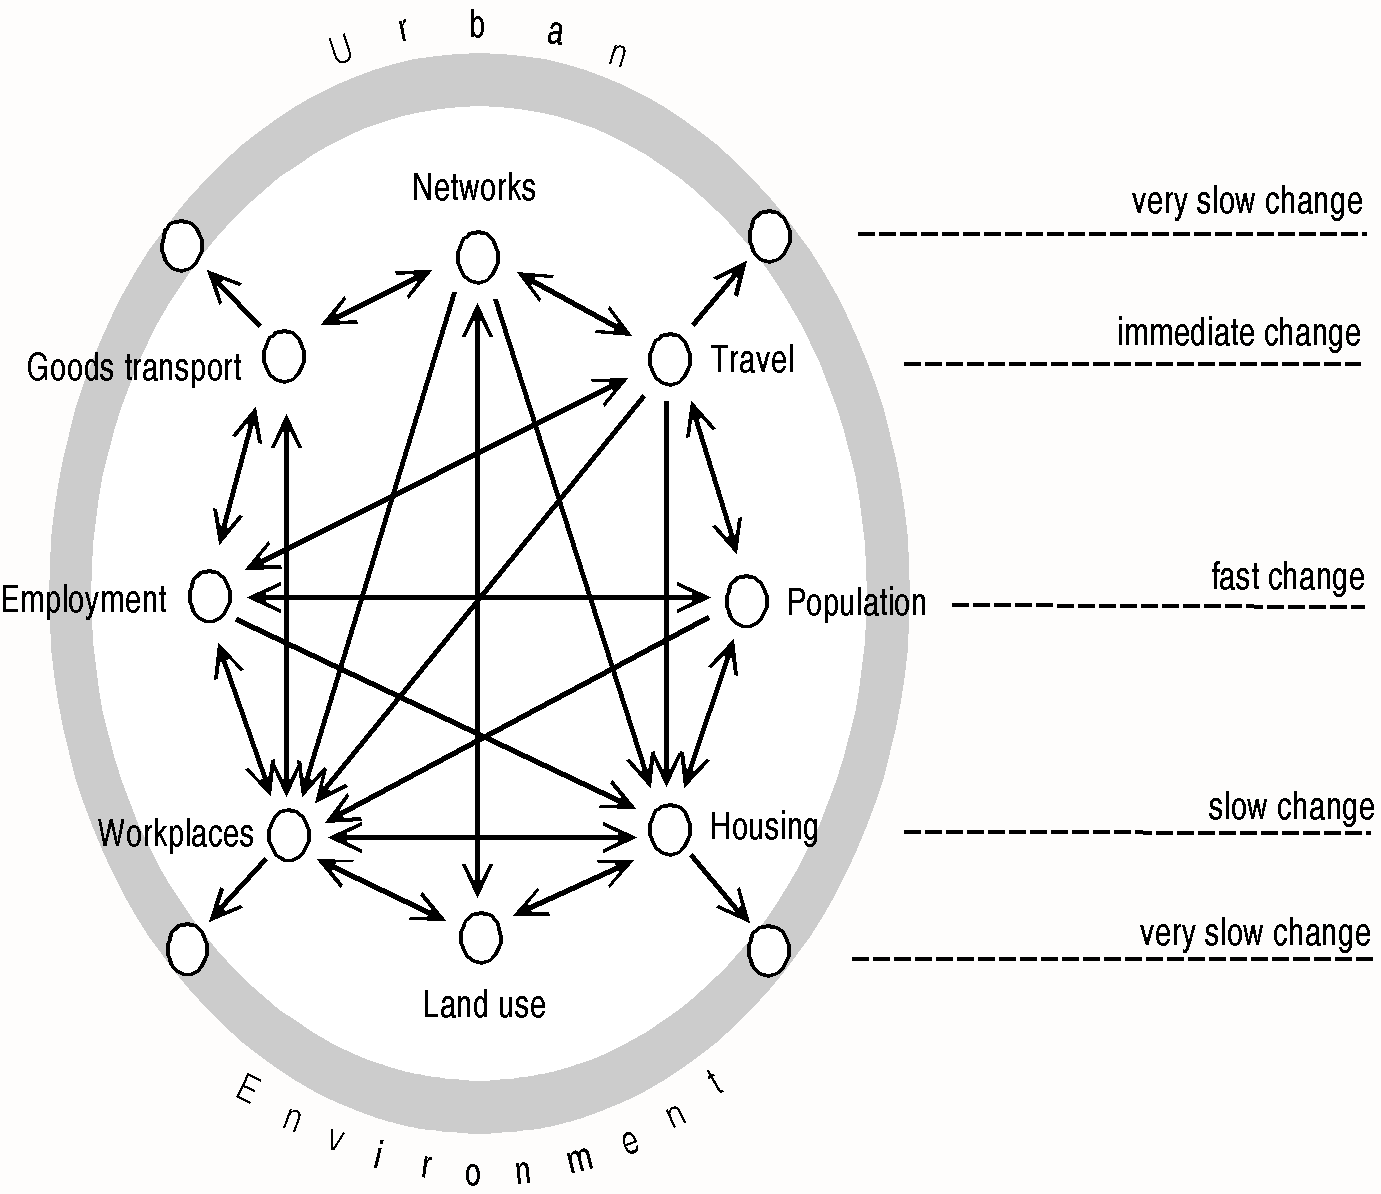
\includegraphics[width=4.5in]
 {wegener.png}
\caption{Web of Urban Processes, from \cite{wegener-1994}}
\label{fig:wegener}
\end{figure}

For the purposes outlined earlier in the paper, the scope of
engodeneity is well represented in Figure \ref{fig:wegener}. These
processes are the central ones in focus, and other processes are
implicated only as needed to adequately represent these.

It is likely that failure to represent almost any of the nodes in
this Figure will induce a significant degree of endogeneity bias
with respect to evaluating urban policies that deal with any of
the nodes.  That is to say, if we assume any of the nodes to be
exogenous, and either leave it out of the model entirely (a gross
misspecification) or assume it is not influenced by feedback from
other nodes we are considering, then our conclusions are
potentially significantly biased by this omission. For a thorough
explanation of the statistical properties of endogeneity bias and
methods to test for the presence of such bias in standard
statistical models, see Greene's treatment of the subject
\cite{greene-2002}.

In the development of UrbanSim to date, the transportation
components represented in the figure are included by loose
coupling to an external travel model system, and the
specifications of the travel model depend on the particular
metropolitan area.  It is common in current-generation
transportation models that goods transport is poorly incorporated
or not included at all, raising a potential source of bias.  This
may be one of the most innocuous of the sources of endogeneity
bias, as others addressed below are likely to have a greater
distorting effect on system behavior.

To address the complexity of the endogenous processes and their
interactions, we have taken into consideration the time scales of
the process to partition processes.  Travel behavior is modelled
(by a loosely coupled travel model system) as a within-day set of
processes, which treat the spatial distributions of activities and
real estate as exogenous, or fixed for the period of the day.
Similarly, we model the location choices of households and firms
within a period we refer to as the short-term (typically defining
this to be more than one day but less than one year).  Short-term
processes treat long-term processes (anything more than a year) as
exogenous - which means the supply side of the real estate market
operates at a long-term scale, while the demand-side operates at a
short-term scale.  Processes that occur within the short-term are
separated from each other by imposing an assumption of limited
information, myopic behavior.  In other words, we avoid the
assumption that agents each know what all other agents are going
to do in the short-term, and optimize their choices based on a
competitive game.  Nor do we impose the assumption that all
processes arise from individual agent-agent interactions. Instead,
we assume that agents make individual choices using limited
information from the past period to form their expectations about
the present and future. These temporal-partitioning and myopic
information assumption allows the model system to be constructed
in a very modular way, minimizing the need for individual
agent-agent interaction or perfect foresight assumptions. These
assumptions (and other design choices) distinguish the UrbanSim
modelling approach from those used in most multi-agent simulation
frameworks such as SWARM, RePast, Ascape and other multi-agent
systems.


\subsection{Endogenous Modelling Boundary}
The spatial extent of the processes considered endogenous is
determined fairly imperfectly based on planning area boundaries
that tend to use official building geographic blocks such as
Counties, and group these into metropolitan regions based on the
degree of social and economic integration, as evidenced in
commuting patterns.  In an ideal situation, the study area
boundary would clearly differentiate one metropolitan study area
from another.  Clearly there are many cases that seriously violate
the assumption that the area outside the boundary does not
significantly influence the internal processes within the study
area.  Almost any metropolitan area on the eastern coast of the
United States, and most in western Europe, are close enough to
each other that the degree of commuting and economic exchange
among them is quite high.  This is the first major endogeneity
bias we must confront.

As the design of UrbanSim is focused on the spatial processes
within a metropolitan region, the boundary effects caused by
metropolitan spillovers surfaces a larger problem, which is that
macro-scale processes are currently handled by loose-coupling to
macro-economic models, but only in the direction from macro-scale
to micro, and not in the reverse direction. This means that local
processes cannot induce changes in the macro-economy, a
potentially significant omission. In particular, it means that two
kinds of policy effects are not currently possible to measure, by
construction.  First is the aggregate economic effect of a major
infrastructure project or other policy. Some of these projects are
arguably large enough to induce measurable macro-scale effects,
such as a new airport. Others, such as localized zoning policies,
would be quite unlikely to induce macro-scale effects on economic
growth.  Second, some policies such as urban growth boundaries or
impact fees have been argued in the literature to potentially
produce enough inflation in housing prices to induce businesses
and households to consider alternative metropolitan locations.  If
there are other metropolitan areas within plausible commuting
distance, this could produce a measurable displacement and trigger
increases in between-metropolitan travel.

How significant this source of endogeneity bias is, and whether it
is large enough to seriously distort the conclusions of an
analysis of local land use, transportation, or environmental
policies, is an open research question.  Certainly, if possible,
it should be addressed in further refinement of the model system,
but it will require integrating macro-scale processes and their
interaction with surrounding metropolitan areas.  We will leave
this particular area of further development to a future paper.

\subsection{Endogenous Market Clearing and Prices}

A major endogeneity issue arises in the context of location
choice, due to the need to reconcile the choices made by locating
agents with the fixed available supply of real estate at those
locations. We shall refer to this in general as a \emph{market
clearing} process, but only in the limited sense that we impose
the accounting constraint that once a location (housing unit) is
chosen by an agent, it is occupied and not available to another
agent until it is vacated by the first.  This means that there
will often be a scarcity of housing at more desirable locations,
and there must be some means to ration the scarce housing among
the agents that wish to locate in them. The assumption of a fixed
supply (stock) of housing in the short-run is equivalent to
assuming that if a household is looking for a house this month,
they cannot contract to have a house built and made available for
them next month.  The time frame for housing supply, as noted
earlier, is considerably longer than the time scale for
residential location choice.

The process currently used in UrbanSim, described in Figure
\ref{fig:choiceprocess}, deals explicitly with the market clearing
constraint imposed by having a fixed supply of housing in the
short-run time frame in which households are making a location
choice.  The market clearing process as currently modelled assumes
that the scarcity of housing at any given location is rationed
according to a randomized order, first-come-first-served process,
not unlike a lottery for the available houses.  It is certainly
not difficult to draw on experience to confirm that there is a
strong degree of random, but sequential, dependence in the way the
housing market works. If person A arrives first and makes a
successful bid on a house, it is not available to person B, even
if the latter would be willing to pay more.

A visual example of the current algorithm makes the process
clearer. Let us simplify the situation to one in which there are
16 neighborhoods, arranged in a rectangular grid.  Assume that
they have 10 houses in each and that there are exactly 160
identical households looking for housing.  Assume further that the
attractiveness of the neighborhoods varies in a systematic way:
cells in the corners have the least attractiveness (1), those on
the edge and not in the corners have an attractiveness of (2), and
those in the center have the highest attractiveness (3).  Note
that the utility is defined as the exponentiated value of these
attractiveness terms, and it is the relative utility that directly
influences choice probabilities.

Figure \ref{fig:grid1} below shows the attractiveness (a), sums of
the individual choice probabilities (b), the count of choices made
by this sample of 160 households on this particular draw of random
numbers \footnote{Note that with a relatively small number of
observations the sum of the choice probabilities differs
significantly from the choice counts due to simulation randomness.
This simulation error diminishes as the number of observations
increases.} (c), and the excess demand in those cells that the
counts exceed housing supply (d).  The excess demand would be the
number of households forced to make a second-best choice from the
remaining available housing, and this would proceed until all
households are placed, provided that there is available housing.
In this example, it would mean that each cell would end up with 10
households, though many would have preferred to locate in the
center cells.

The endogeneity concern in market clearing is twofold.  First,
even though housing prices are included in the utility function,
they are updated only between one simulation year and the next,
and do not dynamically change during a simulation year.  This
places all of the burden of rationing the scarce housing supply
within a simulation year on the lottery process described here,
which may not give enough weight to the role of competitive
bidding in a tight housing market.  On the other hand, it is not
apparent that the market works as a perfectly-informed and
efficient instrument, either. It is implausible to assume that all
households participate in a single massive auction, and each
obtains the house they most prefer, subject to budget constraints,
in a competitive bidding process.  It is more likely that the
random arrival and bidding processes are both facets of the actual
operation of the market.

\begin{figure}[h]
\centerline{
 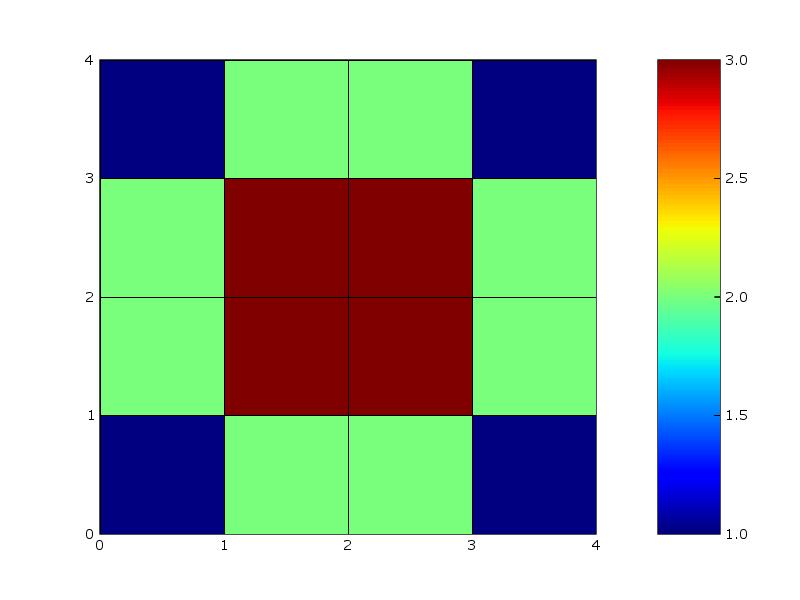
\includegraphics[width=.45\textwidth,height=0.35\textwidth]
 {example_grid_util.png} \hspace{1cm}
 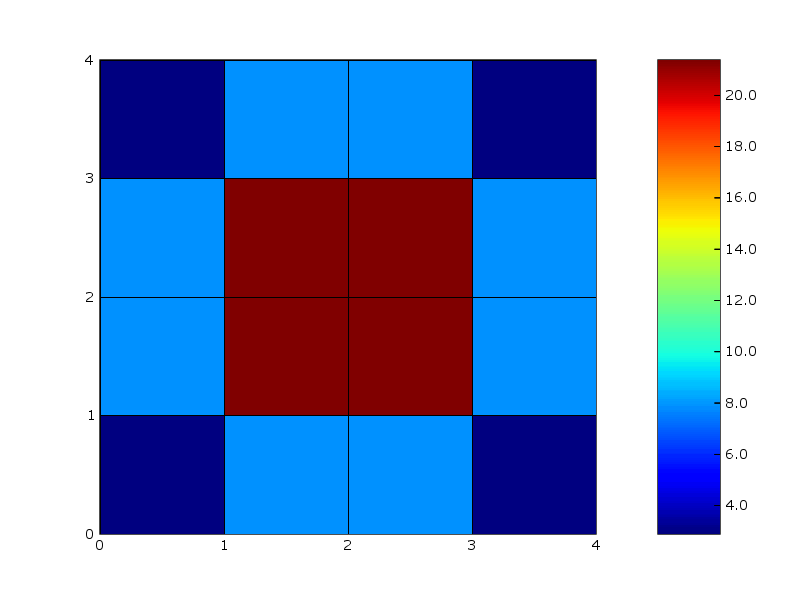
\includegraphics[width=.45\textwidth,height=0.35\textwidth]
 {example_grid_prob.png}}
\end{figure}

\begin{figure}[h]
\centerline{
 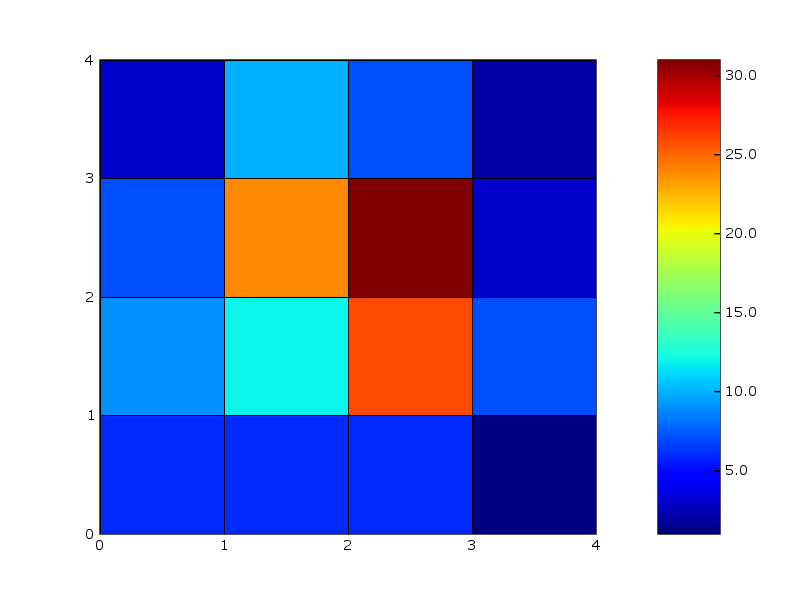
\includegraphics[width=.45\textwidth,height=0.35\textwidth]
 {example_grid_count.png} \hspace{1cm}
 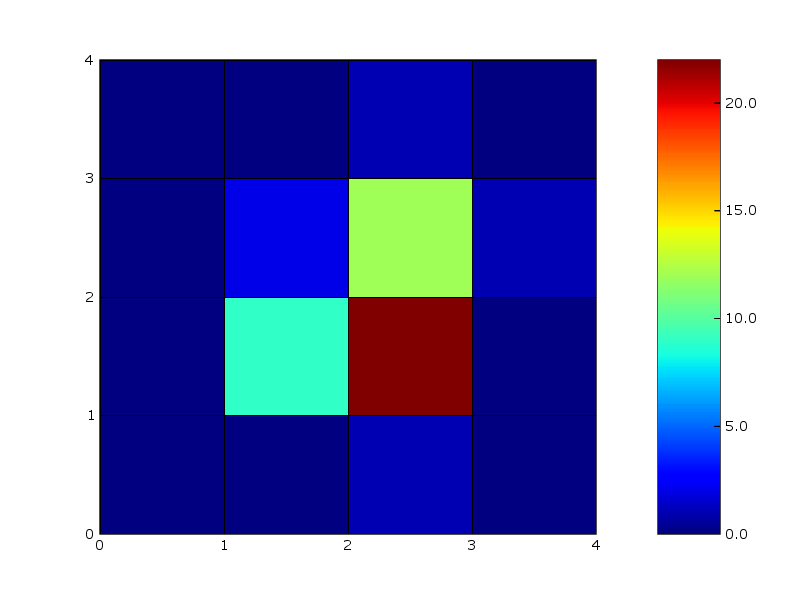
\includegraphics[width=.45\textwidth,height=0.35\textwidth]
 {example_grid_excess.png}}
\caption{\label{fig:grid1} Choice Model Predictions With Limited
Housing}
\end{figure}

\begin{tabbing}
------- \= ------------------------------------------------------------ \= \kill
\> (a) Attractiveness (log(Utilities))  \> (b) Sum of
Probabilities \\  \> (c) Choices (among 160 choosers) \> (d)
Excess Demand
\end{tabbing}


To address these concerns we propose to modify the choice
algorithm shown in Figure \ref{fig:choiceprocess} in two ways. The
first is to simulate the role of a 'landlord' agent in each
neighborhood who monitors market conditions and attempts to
maximize profit by adjusting prices. Depending on how elastic the
demand is, due to substitution possibilities among alternative
neighborhoods, a landlord would increase prices in the presence of
multiple offers in order to increase profit, and lower prices if
the number of offers falls well below the number of housing units
available in the neighborhood.  This would be implemented as an
iterative loop at the choice stage, with landlords updating prices
to improve profits, and households altering their choices in the
face of modified prices.  Notice that both of these agent
responses are consistent with expected behavior, intuitively and
theoretically, and both work to restore balance between demand and
supply.  The revised algorithm is shown in Figure
\ref{fig:choiceprocess2}.

\begin{figure}[h]
\center
 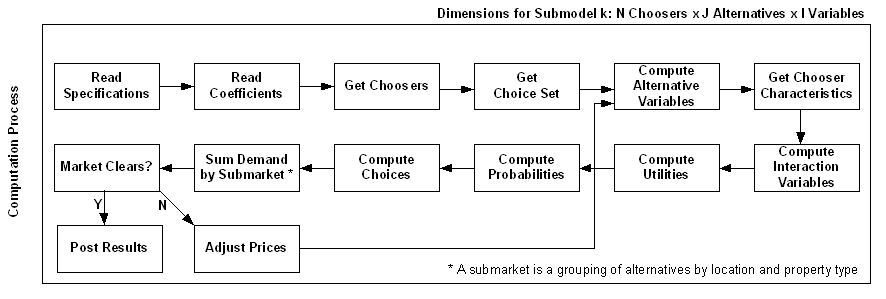
\includegraphics[width=6.5in]
 {ChoiceProcessWithPriceAdjustment.png}
\caption{Choice Process in UrbanSim Location Choice Models}
\label{fig:choiceprocess2}
\end{figure}


The second proposed change is to add a method to the algorithm to
allow the relative weight of the price adjustment process and the
lottery process to vary depending on parameters derived from model
calibration against observed data.  It should be possible to avoid
imposing an arbitrary assumption that only the price mechanism or
only the lottery mechanism are at work, and it should also be
possible to learn the mixture of these processes by examining
observed data.  This modification will require a respecification
of the logit model to include both a constraint and a price
effect.


\subsection{Endogenous Neighborhood Composition}
The literature on residential location choice contains several
streams of research on aspects that link the choices made by
individual households to the aggregate spatial patterns that
emerge.  The feedback between the aggregate patterns and the
individual choices is a major endogeneity concern in most of this
literature.  If the social composition of a neighborhood selection
is valued by a locating household, and the outcome of their
residential location choice changes the social composition of the
neighborhood they locate in, then the individual choice process
and the neighborhood composition are endogenous.

One approach to this endogeneity was first developed by Thomas
Schelling \cite{schelling-1969,schelling-1971,schelling-1978}.
This approach and its extensions simulates the relocation choices
of individual agents based on their satisfaction with the social
composition in their localized neighborhood. Schelling's early
model of residential segregation has inspired considerable
extension in the multi-agent simulation literature.  Its
attractiveness, and the attraction of more recent work on this
approach, derive in no small measure from its transparent
simplicity.  The utility function is essentially due to a single
factor, there are no costs to changing locations, and no
constraints on doing so.

Adding complexity to the utility function, and imposing accounting
constraints on housing supply and a market clearing process as
discussed in the preceding section would makes this modelling
approach considerably less elegant, and possibly less informative.
More problematic from a practical perspective is that there is
considerable computing overhead to processing all agent choices as
localized interactions of agents.  Scaling the model from a small
hypothetical situation to modelling metropolitan regions the size
of Paris, with 11 million inhabitants, or even Seattle, with 3
million, would not be practical on generally-available computers.
Last, it seems likely that localized interactions are insufficient
to capture the rich variety of information flow that informs agent
choices.  Information about housing market opportunities for
example may come from a newspaper or web site, personal experience
such as seeing a for sale or rent sign while travelling through a
neighborhood, information from a social network, or from a real
estate broker.

The approach we have used in UrbanSim to model endogenous
neighborhood composition is to include in the utility function
interaction terms between household characteristics and social
characteristics of the location, and to use a sample of recent
movers to estimate the household location choice model.  The
household characteristics used in UrbanSim include race, household
income, age of head, presence of children, number of persons,
number of workers, and number of vehicles.  Since the model uses
full enumeration of the households, generating compositional
measures using these characteristics is straightforward. What is
less straightforward is the choice of which interaction terms to
include in the utility function, and what spatial frames to use
for the measurement of the social composition effect.  To date,
only a small subset of the possible interaction terms have been
tested in the model system, though the framework and data exist to
test any of the others.

The spatial frame for measuring effects is challenging because of
the theoretical and empirical limitations in our understanding of
neighborhoods and neighborhood effects.  It is clear that defining
neighborhoods is a problematic exercise, since residents often
disagree about or do not know the boundaries of their
neighborhoods, and that the frames of reference differ depending
on the issue at hand: for example shopping for groceries or
choosing a high school.  Moreover, the use of fixed-boundary
neighborhoods can give rise to boundary problems and to potential
for the Modifiable Aerial Unit Problem (MAUP)
\cite{openshaw-taylor-1981}.

For these reasons, we have opted to make the selection of spatial
frames of reference as flexible as possible, using grid cells as
the low-level spatial building block. Figure \ref{fig:gridmap}
shows the relative scales of 150 meter grid cells in central
Seattle to Traffic Analysis Zone (TAZ) and Forecast Analysis Zone
(FAZ) geographies used in transportation modelling, and to
underlying land ownership parcels.  The spatial frames of
reference available in UrbanSim to measure compositional effects
are the following:

\begin{itemize}

\item Grid cell (user-definable, but typically 150 by 150 meters)
\tight

\item Radius Surrounding Grid Cell (user-definable, typically 600
meters)

\item Traffic Analysis Zone (used in transportation modelling)

\item Census Block, Census Block Group, or Census Tract

\item City

\item County

\item Any Geography that is Assigned to Gridcells

\item Dynamically Updated Boundaries Assigned to Gridcells
\footnote{The use of statistical classification techniques to
generate typologies of neighborhoods is being explored in
UrbanSim, but currently requires some coding to implement.}

\end{itemize}


\begin{figure}[h]
\centerline{
 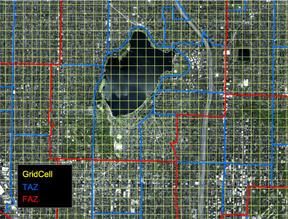
\includegraphics[width=.45\textwidth,height=0.35\textwidth]
 {gridmap2-small.png} \hspace{1cm}
 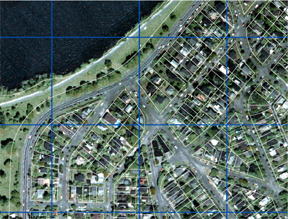
\includegraphics[width=.45\textwidth,height=0.35\textwidth]
 {gridmap-small.png}}
\caption{\label{fig:gridmap} 150 x 150 Meter Grid Cells in Central
Seattle}
\end{figure}

Compositional variables may be used at different scales, depending
on the nature of their effects, and there is no restriction on the
mixing of multiple scales.  This opens the possibility for
developing multi-level models that address the correlations among
multiple scales.  See for example, \cite{goldstein-book-1995} for
a thorough introduction to this topic.

In the application of UrbanSim in the Puget Sound region of
Seattle, Washington, the household location choice model was
estimated using a stratification of households by age and size, to
allow measurement of life cycle effects on the preferences of
households for locational characteristics.  Income and presence of
children were also used in the specification, but as interaction
terms.  Variables used in the Puget Sound household location
choice model are defined in Table \ref{tab:vardef}.  Model
estimation results using a sample of 2,364 households who moved
between 1995 and 2000 are given in Table \ref{tab:hlc}.

\begin{table}[h]
\caption{Variables Used in Household Location Choice Model, Puget
Sound Region} \label{tab:vardef}
\centering
\begin{tabular}{ll}
\hline\hline
BCOS\_IN & Annualized Cost of Housing / Household Income \\
BDUR\_C & Dwelling Units in Cell * Has Children Dummy \\
BART & Close to Arterial Dummy \\
BINCIVAL & Income * Improvement Value per Unit \\
BLDUW & Log of Dwelling Units within 600 Meters \\
BPHIW\_H & High Income Dummy * Pct High Income in 600 Meters \\
BPMIW\_M & Middle Income Dummy * Pct Middle Income within 600
Meters \\
BPLIW\_L & Low Income Dummy * Pct Low Income Within 600 Meters
\\
BPMNWMJ & Minority Dummy * Pct Minority Within 600 Meters
\\
BPMNWMN & White Dummy * Pct Minority Within 600 Meters \\
BSAGEFAZ & Number of Households in FAZ of Same Age Category as
Household \\
SSIZFAZ & Number of Households in FAZ of Same Size Category as
Household \\
BYH\_HDR & Young Household Head (< 40) * High Density Residential
\\
YH\_M & Young Household Dummy * Mixed Use \\
BHBWUSO & Utility of Travel to Work by Auto \\
BHBWUTW & Utility of Travel to Work by Transit \\

\hline
\end{tabular}
\end{table}

The cost to income ratio provides an interaction that captures
price effects on location choice.  It is expected have a negative
sign, meaning that households prefer spending a smaller fraction
of their income on housing if presented with two alternatives that
are the same on all other measured characteristics except cost.
The results are all negative, and significant for all except young
single-person and 3+ person households.

The interaction of income of household with the percentage of
households of the same income tercile within the area within
walking distance (600 meters) are significant and positive for
only 6 of the 18 parameters estimated (3 parameters for 6 types of
households), with the strongest positive effects for younger
households with 3 or more persons.

The interaction between minority households and the percent
minority within walking distance was positive for all but young
one-person households, and significant for all households with at
least 2 persons.  White households had negative and significant
coefficients on the percentage minority within walking distance in
all six household types.

Age clustering was tested with the same age in FAZ (a proxy for
larger neighborhood) but found to be significant only for young
singles, not an entirely surprising result.  Younger households
and those without children also showed quite different preferences
for urbanization, as measured by transit utility and density of
housing in a cell, with a greater affinity to areas with high
transit utility and higher density.

The interactions of household characteristics and social
composition of neighborhoods, measured at scales from the grid
cell, to walking distance, to larger FAZ geographies, measure the
degree to which neighborhood composition influences individual
choice of residence location.  After households make choices and
locate in specific cells over the course of an annual simulation
step, the composition of each neighborhood is updated, and these
new compositions influence choices in the subsequent year. This
process represents the feedbacks between individual choice and
neighborhood composition, but there is still considerable room for
improvement.

One of the first improvements that can be made is to address the
market clearing endogeneity concerns outlined in the preceding
section, as these will interact with the neighborhood composition
concerns.  For example, if the current algorithm relies
unrealistically on a lottery process for market clearing, it is
likely to cause excessive diffusion in spatial concentrations of
social groups over time.

Two potentially confounding specification issues that warrant
further investigation are the role of taste heterogeneity and of
unmeasured quality variations that are correlated with price.  In
a stream of research pioneered by Berry, Levinsohn and Pakes in
1995, there has been a growing body of research dealing with the
specification and estimation of choice models with unmeasured
quality and taste heterogeneity
\cite{berry-econometrica-1995,berry-cowles-2003}. Initially
focused on the automobile market, this research has recently
expanded to address the housing market, neighborhood sorting and
segregation. It suggests that failure to account for taste
heterogeneity and unmeasured quality variation correlated with
price could bias parameter estimates significantly. Testing these
specification concerns in the context of UrbanSim remains for
future research.


\section{Conclusions}

Endogeneity is a serious challenge to successful modelling of
urban social dynamics.  In the design of UrbanSim we have
addresses with reasonable success the treatment of engogeneity of
modelling scope, particularly through the decoupling of processes
that run at different time scales, but also by using assumptions
about information that are neither entirely local, nor perfectly
informed about the present and future.  Endogeneity of modelling
boundary has been handled only indirectly by delegation to a
loosely-coupled macro-economic model, but this is not completely
satisfactory as it is only a top-down feedback now.  Future work
should address this limitation.

The two sources of endogeneity dealt with in more detail are those
associated with location choice, endogeneity of market clearing
and endogeneity of neighborhood composition. Regarding the first,
there is clearly a need to balance the roles of random aspects
that arise from random sequencing of location choices with the
role of price adjustment through a competitive process or a
supply-side (landlord) adjustment.  These need further development
in future research.  Regarding the second, much has been done
already to incorporate neighborhood composition effects, at
multiple levels, with and without fixed boundaries.  More remains
to be done, especially by exploring specifications that allow for
measuring taste heterogeneity and unmeasured quality variations
that are correlated with price, which could cause endogeneity
bias.

One of the main steps being taken to facilitate these next
advances is the re-engineering of the UrbanSim software platform.
It is being ported from Java to Python, using numeric libraries,
to increase speed, modularity, and productivity in code
development.  A broad international group of research teams is
beginning to collaborate around the development of this platform,
under the working name of Open Platform for Urban Simulation
\footnote{A preliminary website has been set up to provide access
to software developed by the project, and the first release is
expected some time in 2005.  See www.opus-network.org}.

\vspace{1cm} {\bf \large Acknowledgments}

The research described in this paper has been funded principally
by grants from the National Science Foundation Grants EIA-0121326
and BCS-0120024, and the Puget Sound Regional Council.

\clearpage
\begin{table}[h]
\caption{Estimation Results for Household Location Choice Model,
Puget Sound Region} \label{tab:hlc} \centering
\begin{tabular}{lrr|rr|rr}
\\
Age 40 or Less  &   \multicolumn{2}{c}{1 Person}  &
\multicolumn{2}{c}{2 Person}   &   \multicolumn{2}{c}{3 or More Persons}    \\
\hline\hline & beta & b./std. err & beta & b./std. err & beta &
b./std. err \\
BCOS\_IN &   -0.2557 &   -1.63   &   -1.7230 &   -4.74   &   -0.1572 &   -1.20   \\
BDUR\_C  &       &       &   -0.0122 &   -2.24   &   -0.0111 &   -5.14   \\
BART    &   0.2072  &   1.44    &   0.0684  &   0.49    &   -0.1166 &   -1.00   \\
BINCIVAL    &   0.0000  &   1.28    &   0.0000  &   5.54    &   0.0000  &   6.36    \\
BLDUW   &   0.3763  &   3.18    &   0.2172  &   2.08    &   0.2857  &   4.16    \\
BPHIW\_H &   0.0381  &   2.66    &   0.0080  &   0.81    &   0.0144  &   2.07    \\
BPMIW\_M &   0.0164  &   1.59    &   0.0166  &   1.76    &   0.0267  &   4.19    \\
BPLIW\_L &   0.0214  &   2.50    &   -0.0016 &   -0.14   &   0.0185  &   2.34    \\
BPMNWMJ &   -0.0021 &   -0.18   &   0.0312  &   2.50    &   0.0225  &   2.39    \\
BPMNWMN &   -0.0152 &   -2.58   &   -0.0188 &   -3.12   &   -0.0182 &   -3.80   \\
BSAGEFAZ    &   0.0005  &   3.66    &   0.0002  &   1.67    &   0.0000  &   0.29    \\
SSIZFAZ &   -0.0001 &   -1.68   &   0.0000  &   -0.27   &   0.0002  &   1.87    \\
BYH\_HDR &   0.4440  &   1.53    &   0.5632  &   2.29    &   0.3565  &   1.98    \\
YH\_M    &   0.4582  &   1.46    &   0.7549  &   2.79    &   0.6555  &   2.88    \\
BHBWUSO &   1.2211  &   0.87    &   1.0097  &   0.83    &   2.8577  &   3.74    \\
BHBWUTW &   13.1195 &   1.61    &   14.2051 &   1.88    &   -22.7206    &   -3.63   \\
\hline \\
Age Over 40 & \multicolumn{2}{c}{1 Person}   &
\multicolumn{2}{c}{2 Person}   &     \multicolumn{2}{c}{3 or More Persons}    \\
\hline
BCOS\_IN &   -0.9677 &   -4.68   &   -0.8034 &   -2.97   &   -1.1394 &   -2.50   \\
BDUR\_C  &       &       &       &       &   -0.0150 &   -3.58   \\
BART    &   0.2878  &   2.16    &   0.1349  &   0.97    &   0.1930  &   1.13    \\
BINCIVAL    &   0.0000  &   2.93    &   0.0000  &   7.02    &   0.0000  &   6.08    \\
BLDUW   &   0.2436  &   2.37    &   0.1162  &   1.39    &   0.2166  &   2.21    \\
BPHIW\_H &   0.0168  &   1.11    &   0.0139  &   1.71    &   0.0108  &   1.32    \\
BPMIW\_M &   0.0096  &   0.93    &   0.0132  &   1.52    &   0.0123  &   1.27    \\
BPLIW\_L &   0.0165  &   2.14    &   0.0029  &   0.30    &   -0.0019 &   -0.13   \\
BPMNWMJ &   0.0117  &   0.68    &   0.0590  &   3.50    &   0.0405  &   2.68    \\
BPMNWMN &   -0.0255 &   -4.22   &   -0.0117 &   -2.03   &   -0.0313 &   -3.85   \\
BSAGEFAZ    &   0.0002  &   1.37    &   0.0002  &   0.79    &   -0.0002 &   -0.87   \\
SSIZFAZ &   0.0000  &   -0.50   &   -0.0001 &   -0.45   &   0.0004  &   2.10    \\
BHBWUSO &   2.7715  &   2.28    &   3.3305  &   3.42    &   1.7744  &   1.55    \\
BHBWUTW &   12.7920 &   1.58    &   -9.5427 &   -1.28   & -13.4521 &   -1.38 \\
\hline\hline

\end{tabular}

\end{table}
\clearpage



Leigh Tesfatsion, "Agent-Based Computational Economics: A
Constructive Approach to Economic Theory"  (pdf preprint, 253K),
Chapter 1 in Leigh Tesfatsion and Kenneth L. Judd (Eds.), Handbook
of Computational Economics, Vol. 2: Agent-Based Computational
Economics   (Table of Contents and Abstracts), Handbooks in
Economics Series, North-Holland/Elsevier, Amsterdam, 2006, to
appear.




\bibliography{urbansim}
\bibliographystyle{plain}
\end{document}
